\documentclass[12pt]{article}
\usepackage[margin=1in]{geometry} 
\usepackage{amsmath,amsthm,amssymb,amsfonts}
\usepackage{enumerate,listings,graphicx,epstopdf,siunitx}
\usepackage{color}
\graphicspath{~/Documents/school/fall16/stat586/hw5}

\sloppy
\definecolor{lightgray}{gray}{0.5}
 
\newcommand{\N}{\mathbb{N}}
\newcommand{\Z}{\mathbb{Z}}
\newcommand{\normD}[3]{\frac{1}{\sqrt{2\pi #1^2}}exp(\frac{-( #2 - #3)^2}{2 #1^2})} 
\newenvironment{problem}[2][Problem]{\begin{trivlist}
\item[\hskip \labelsep {\bfseries #1}\hskip \labelsep {\bfseries #2.}]
  \vspace{1 cm}
}{\end{trivlist}}

\begin{document}
\title{Homework Set 5}
\author{Taylor Bodin}
\maketitle

\section*{Problem 5.1}
\subsection*{a.}
\[P(x<\frac{3}{4}) = F_{X,Y}(\frac{3}{4},\infty) = \frac{3}{4} \]

\subsection*{b.}
\[P(x>\frac{1}{2}) = 1 - F_{X,Y}(\frac{1}{2},\infty) = 1 - \frac{1}{2} = \frac{1}{2} \]

\subsection*{c.}
\[P(y>\frac{1}{4}) = 1 - F_{X,Y}(\frac{1}{4},\infty) = \frac{3}{4} \]

\subsection*{c.}
\[P(\frac{1}{4}<x<\frac{1}{2},\frac{1}{2}<y<1) = F_{X,Y}(\frac{1}{2},1)-F_{X,Y}(\frac{1}{4},\frac{1}{2}) 
= \frac{1}{2}(1)-\frac{1}{2}\frac{1}{4} = \frac{3}{8} \]

\section*{Problem 5.3}
\subsection*{Setup}
\subsubsection*{Determine the Coefficients}
\begin{align*}
F_{X,Y}(0,0) &= 0 = 1 - ae^0 - be^0 + ce^0 = 1 - a - b + c \\
F_{X,Y}(0,\infty) &= 0 = 1 - ae^0 = 1 - a  \\
F_{X,Y}(\infty,0) &= 0 = 1 - be^0 = 1 - b & & \textrm{Solving the system yields} \\
a &= b = c = 1
\end{align*}

\subsubsection*{Determine $F_X(x)$}
\[F_X(x) = F_{X,Y}(x,\infty) = 1-e^{-x}\]

\subsubsection*{Determine $F_Y(y)$}
\[F_Y(y) = F_{X,Y}(\infty,y) = 1-e^{-y}\]

\subsection*{a.}
\[P(a<X<b) = F_X(b) - F_X(a) = (1-e^{-b})-(1-e^{-a}) = e^{-a}-e^{-b}\]

\subsection*{b.}
\[P(c<X<d) = F_X(d) - F_X(c) = (1-e^{-d})-(1-e^{-c}) = e^{-c}-e^{-d}\]

\subsection*{c.}
\begin{align*}
  P(a<X<b|c<X<d) &= \frac{F_{X,Y}(b,d)-F_{X,Y}(b,c) - F_{X,Y}(a,d) + F_{X,Y}(a,c)}
    {e^{-c}-e^{-d}} & & \textrm{everything cancels except} \\
    &= \frac{e^{-(b+d)}-e^{-(b+c)}-e^{-(a+d)}+e^{-(a+c)}}{e^{-c}-e^{-d}} \\
\end{align*}

\subsection*{Statistical Independance}
X and Y are statistically independant if, $P(a<X<b|c<X<d) = P(a<X<b)$ \\
\begin{align*}
e^{-a}-e^{-b} &= \frac{e^{-(b+d)}-e^{-(b+c)}-e^{-(a+d)}+e^{-(a+c)}}{e^{-c}-e^{-d}} \\
(e^{-a}-e^{-b})(e^{-c}-e^{-d}) &= e^{-(b+d)}-e^{-(b+c)}-e^{-(a+d)}+e^{-(a+c)} \\
e^{-(b+d)}-e^{-(b+c)}-e^{-(a+d)}+e^{-(a+c)} &= e^{-(b+d)}-e^{-(b+c)}-e^{-(a+d)}+e^{-(a+c)}, & & \textrm{QED} \\
\end{align*}

\section*{Problem 5.5}
\begin{align*}
  P(a<X<b)P(c<Y<d) &= P(a<X<b,c<Y<d) \\
  &= F_{X,Y}(b,d)-F_{X,Y}(b,c)-F_{X,Y}(a,d)+F_{X,Y}(a,c) \\
  &= F_X(b)F_Y(d)-F_X(b)F_Y(c)-F_X(a)F_Y(b)+F_X(a)F_Y(c) \\
  &= (F_X(b)-F_X(a))(F_Y(d)-F_Y(c)) \\
  &= P(a<X<b)P(c<Y<d), & & \textrm{QED}
\end{align*}

\section*{Problem 5.7}
\subsection*{a.}
d has to satisfy the following inequality: $0\leq d \leq (ax+by+c)^n$

\subsection*{b.}
\subsubsection*{$f_X(x)$}
\[f_x(x) = \int_0^\infty \frac{d}{(ax+by+c)^n} dy
  = \frac{-d(by+ax+c)^{1-n}}{b(n-1)}\big|_0^\infty
= \frac{d(ax+c)^{1-n}}{b(n-1)}\]

\subsubsection*{$f_Y(y)$}
\[f_y(y) = \int_0^\infty \frac{d}{(ax+by+c)^n} dx
  = \frac{-d(by+ax+c)^{1-n}}{b(n-1)}\big|_0^\infty
= \frac{d(by+c)^{1-n}}{a(n-1)}\]

\subsection*{c.}
\[\int_0^\infty \int_0^y \frac{d}{(ax+by+c)^n} dxdy 
  = \frac{d}{a(n+1(n+2)}\left[ \frac{c^{2-n}}{b} \frac{c^{2-n}}{a+b}\right]\]

\section*{Problem 5.9}
\subsection*{a.}
\begin{align*}
 f_{r,\theta}(r,\theta) &= 
 \begin{cases}
   c\sqrt{1-r^2}, & r^2 \leq 1 \\
   0, & otherwise
 \end{cases} \\
 1 &= \int_0^{2\pi} \int_0^1 c\sqrt{1-r^2}rdrd\theta \\
 1 &= \frac{2\pi c}{3} \\
 c &= \frac{3}{2\pi c}
\end{align*}

\subsection*{b.}
\begin{align*}
  P(X^2 + Y^2 > \frac{1}{4}) &= \int_0^{2\pi} \int_\frac{1}{4}^1 c\sqrt{1-r^2}rdrd\theta
  &= \frac{15\sqrt{15}}{64} = .9077
\end{align*}

\subsection*{c.}
\begin{align*}
  P(X>Y) &= \int_{\frac{-3\pi}{4}}^{\frac{\pi}{4}} \int_0^1 c\sqrt{1-r^2}rdrd\theta \\
  &= \frac{1}{2}
\end{align*}

\section*{Problem 5.11}
\subsection*{a.}
The area of and ellipse is $ab\pi$ which in this case is $6\pi$. Normalizing by the area:
\[f_{x,y}(x,y) = 
\begin{cases}
\frac{1}{6\pi}, & 9x^2 + 4y^2  < 36 \\
0, & otherwise
\end{cases}
\]
\subsection*{b.}
\subsubsection*{Find $f_x(x)$}
\begin{align*}
  f_x(x) &= \int_{\frac{-\sqrt{36-9x^2}}{4}}^{\frac{\sqrt{36-9x^2}}{4}}\frac{1}{6\pi} dy \\
  &= \frac{1}{2\pi} \sqrt{4-x^2}, & -2 \leq x \leq 2
\end{align*}

\subsubsection*{Find $f_y(y)$}
\begin{align*}
  f_y(y) &= \int_{\frac{-\sqrt{36-4y^2}}{9}}^{\frac{\sqrt{36-4y^2}}{9}}\frac{1}{6\pi} dx \\
  &= \frac{2}{9\pi}\sqrt{9-y^2}, & -3 \leq y \leq 3
\end{align*}

\subsection*{c.}
\subsubsection*{Find $P(X<1)$}
\[P(X>1) = \int_1^2 \frac{1}{2\pi} \sqrt{4-x^2}dx = .1955 \]

\subsubsection*{Find $P(Y<1)$}
\[P(Y<1) = \int_{-3}^1 \frac{2}{9\pi}\sqrt{9-y^2} = .7082 \]

\subsection*{d.}
\[P(Y<1|X>1) = \int_1^{\frac{\sqrt{27}}{2}} \int_{1}^{\frac{\sqrt{36-4y^2}}{9}}\frac{1}{6\pi} = .0468 \]

\section*{Problem 5.13}
\subsection*{a.}
\begin{align*}
  1 &= \sum_{m=0}^{L-1} \sum_{n=0}^{L-1-m} c \\
  &= c\frac{L(L+1)}{2} \\
  c &= \frac{2}{L(L+1)} \\
\end{align*}

\subsection*{b.}
\subsubsection*{Find $P_M(m)$}
\[P_M(m) = \sum_{n=0}^{L-1-m}\frac{2}{L(L+1)}  = \frac{2(L-m)}{L(L+1)} \]

\subsubsection*{Find $P_N(m)$}
\[P_N(n) = \sum_{m=0}^{L-1-n}\frac{2}{L(L+1)}  = \frac{2(L-n)}{L(L+1)} \]

\subsection*{c.}
\begin{align*}
  P(M+N<\frac{L}{2}) = 
  &= \begin{cases}
    \sum_{m=0}^{\frac{L}{2}} \sum_{n=0}^{\frac{L}{2}-m} \frac{2}{L(L+1)}, & L \ \textrm{odd} \\
    \sum_{m=0}^{L\frac{L}{2}-1} \sum_{n=0}^{\frac{L}{2}-1-m} \frac{2}{L(L+1)}, & L \ \textrm{odd} \\
  \end{cases} \\
  &= \begin{cases}
    \frac{(L+2)(L+4)}{4L(L+1)}, & L \ \textrm{odd} \\
    \frac{(L+2)}{4(L+1)}, & L \ \textrm{odd} \\
  \end{cases}
\end{align*}

\section*{Problem 5.15}
\subsection*{a.}
By a geometry, $c = \frac{1}{k^2}$

\subsection*{b.}
\subsubsection*{Find $P_M(m)$}
\[\sum_{n=0}^{k-1}\frac{1}{k^2} = \frac{k}{k^2} = \frac{1}{k}\]

\subsubsection*{Find $P_N(n)$}
\[\sum_{m=0}^{k-1}\frac{1}{k^2} = \frac{k}{k^2} = \frac{1}{k}\]

\subsection*{c.}
\[\sum_{n=0}^{\frac{k}{2}}\sum_{m=0}^{\frac{k}{2}-N}\frac{1}{k^2} = \frac{(k+2)(k+4)}{8k^2}\]

\section*{Problem 5.17}
\subsection*{a.}
\[P(m|n=2) = \begin{cases}
    \frac{4}{7}, & m = 1 \\
    \frac{2}{7}, & m = 2 \\
    \frac{1}{7}, & m = 3 \\
     0, & otherwise
   \end{cases}
\]

\subsection*{b.}
\[P(m|n\geq2) = \begin{cases}
    \frac{14}{24}, & m = 1 \\
    \frac{7}{24}, & m = 2 \\
    \frac{3}{24}, & m = 3 \\
     0, & otherwise
   \end{cases}
\]

\subsection*{c.}
\[P(m|n\neq2) = \begin{cases}
    \frac{14}{31}, & m = 1 \\
    \frac{10}{31}, & m = 2 \\
    \frac{7}{31}, & m = 3 \\
     0, & otherwise
   \end{cases}
\]

\section*{Problem 5.19}
\subsection*{Setup}
The area of this diamond shaped region is 2, therefor the normalizing constant needed for a uniform probability in the region is $\frac{1}{2}$.
Using this constant it's easy to determine the pdf and marginals

\begin{align*}
  f_{x,y}(x,y) &=
  \begin{cases}
    \frac{1}{2}, & |x| + |y| \leq 1 \\
    0, & otherwise
  \end{cases} \\
  f_{x}(x) &=
  \begin{cases}
    x+1, & -1\leq x \leq 0 \\
    -x+1, & 0\leq x \leq 1 \\
    0, & otherwise
  \end{cases} \\
  f_{y}(y) &=
  \begin{cases}
    y+1, & -1\leq y \leq 0 \\
    -y+1, & 0\leq y \leq 1 \\
    0, & otherwise
  \end{cases} \\
\end{align*}
\subsection*{a.}
\subsubsection*{Find $f_{x|y}(x)$}
\begin{align*}
  f_{x|y}(x) &= \frac{f_{x,y}(x,y)}{f_y(y)} \\
  &= \begin{cases}
    \frac{1}{2(y+1)}, & -1 \leq y \leq 0 \\
    \frac{1}{2(-y+1)}, & 0 \leq y \leq 1 \\
    0, & otherwise
  \end{cases} \\
\end{align*} 

\subsubsection*{Find $f_{y|x}(y)$}
\begin{align*}
  f_{y|x}(y) &= \frac{f_{x,y}(x,y)}{f_x(x)} \\
  &= \begin{cases}
    \frac{1}{2(x+1)}, & -1 \leq x \leq 0 \\
    \frac{1}{2(-x+1)}, & 0 \leq x \leq 1 \\
    0, & otherwise
  \end{cases} \\
\end{align*} 

\subsection*{b.}
\subsubsection*{Find $F_{x|y}(x)$}
\begin{align*}
  F_{x|y}(x) &= \frac{\int_{-\infty}^x f_{x,y}(x',y)dx'}{f_y(y)} \\
  &= \begin{cases}
    \frac{x+y+1}{2(y+1)}, & -1 \leq y \leq 0  \\
    \frac{-x+y+1}{2(-y+1)}, & 0 \leq y \leq 1  \\
    0, & otherwise
  \end{cases} \\
\end{align*} 

\subsubsection*{Find $F_{y|x}(y)$}
\begin{align*}
  F_{y|x}(y) &= \frac{\int_{-\infty}^y f_{x,y}(x,y')dy'}{f_x(x)} \\
  &= \begin{cases}
    \frac{x+y+1}{2(x+1)}, & -1 \leq x \leq 0 \\
    \frac{x-y+1}{2(-x+1)}, & 0 \leq x \leq 1 \\
    0, & otherwise
  \end{cases} \\
\end{align*} 

\subsection*{c.}
\subsubsection*{Find $f_{x|y>\frac{1}{2}}(x)$}
\begin{align*}
  f_{x|y>\frac{1}{2}}(x) &= \frac{\int_{\frac{1}{2}}^{|x|+1} f_{x,y}(x',y)dx'}{\int_{\frac{1}{2}}{1}f_y(y)} \\
  &= \begin{cases}
    2(2x+1), & -\frac{1}{2} \leq x \leq 0 \\
    -2(2x+1), & 0 \leq x \leq \frac{1}{2} \\
    0, & otherwise
  \end{cases} \\
\end{align*} 

\subsubsection*{Find $F_{x|y>\frac{1}{2}}(y)$}
\begin{align*}
  F_{x|y>\frac{1}{2}}(y) &= \frac{F_{x,y}(x,y_2)-F_{x,y}(x,y_1)}{F_y(y_2)-F_y(y_1)} \\
  &= \frac{-.25(|x|-x-1)}{\frac{39}{8}}
\end{align*} 

\section*{Problem 5.75}
$c^2$ is the contour level and controls the size of the ellipse \\
$\sigma_x , \sigma_y$ control the axis of the ellipse \\
$\rho_{xy}$ is the correlation coefficient and as it gets bigger it makes the ellipse look
more and more like $x = y$ \\

\subsection*{Setup}

\begin{verbatim}
clear; close all; clc

[X,Y] = meshgrid(-8:0.1:8);
mux = 0; muy = 0;
\end{verbatim}


\subsection*{A}

\begin{verbatim}
stdx = 3; stdy = 3;
varx = stdx^2; vary=stdy^2;
rho = 0;

X1 = (X-mux)/stdx;
Y1 = (Y-muy)/stdy;

Z = X1.^2-2*rho*X1.*Y1+Y1.^2;
c = 1;

figure(1);
contour(X,Y,Z,c)

title('Std x = Std y');
xlabel('x'); ylabel('y');
axis([-9 9 -9 9]);
\end{verbatim}

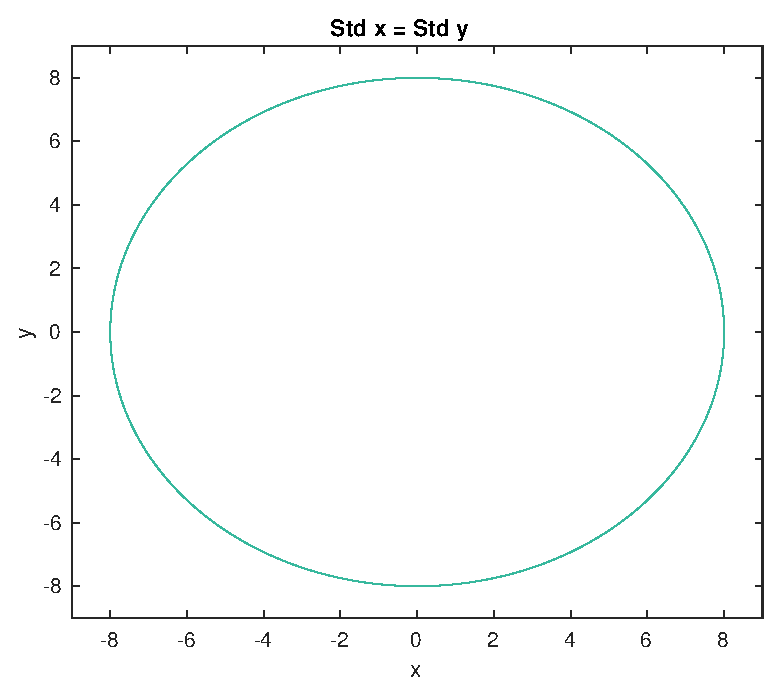
\includegraphics [width=4in]{prob_5_75_01.eps}


\subsection*{B}

\begin{verbatim}
stdx = 1; stdy = 3;
varx = stdx^2; vary=stdy^2;
rho = 0;

X1 = (X-mux)/stdx;
Y1 = (Y-muy)/stdy;

Z = X1.^2-2*rho*X1.*Y1+Y1.^2;
c = 1;

figure(2);
contour(X,Y,Z,c)

title('Std x < Std y');
xlabel('x'); ylabel('y');
\end{verbatim}

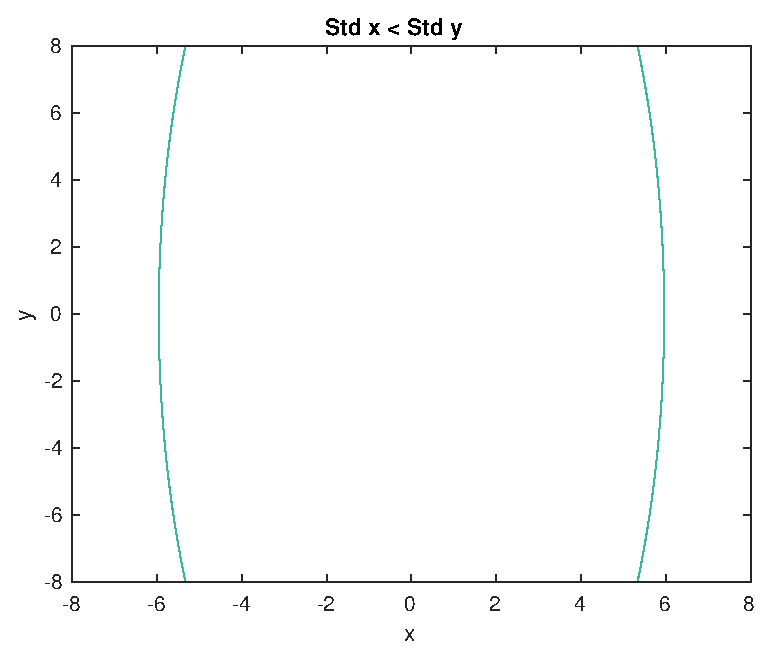
\includegraphics [width=4in]{prob_5_75_02.eps}


\subsection*{C}

\begin{verbatim}
stdx = 3; stdy = 1;
varx = stdx^2; vary=stdy^2;
rho = 0;

X1 = (X-mux)/stdx;
Y1 = (Y-muy)/stdy;

Z = X1.^2-2*rho*X1.*Y1+Y1.^2;
c = 1;

figure(3);
contour(X,Y,Z,c)

title('Std x > Std y');
xlabel('x'); ylabel('y');
\end{verbatim}

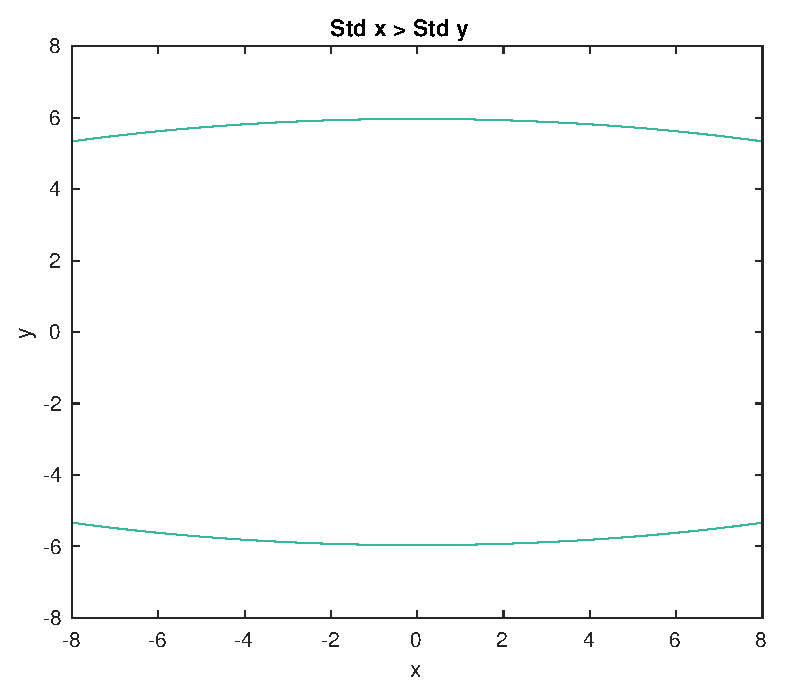
\includegraphics [width=4in]{prob_5_75_03.eps}


\subsection*{D}

\begin{verbatim}
stdx = 3; stdy = 3;
varx = stdx^2; vary=stdy^2;
rho = .5;

X1 = (X-mux)/stdx;
Y1 = (Y-muy)/stdy;

Z = X1.^2-2*rho*X1.*Y1+Y1.^2;
c =1;

figure(4);
contour(X,Y,Z,c)

title('Std x = Std y, Rho != 0');
xlabel('x'); ylabel('y');
\end{verbatim}

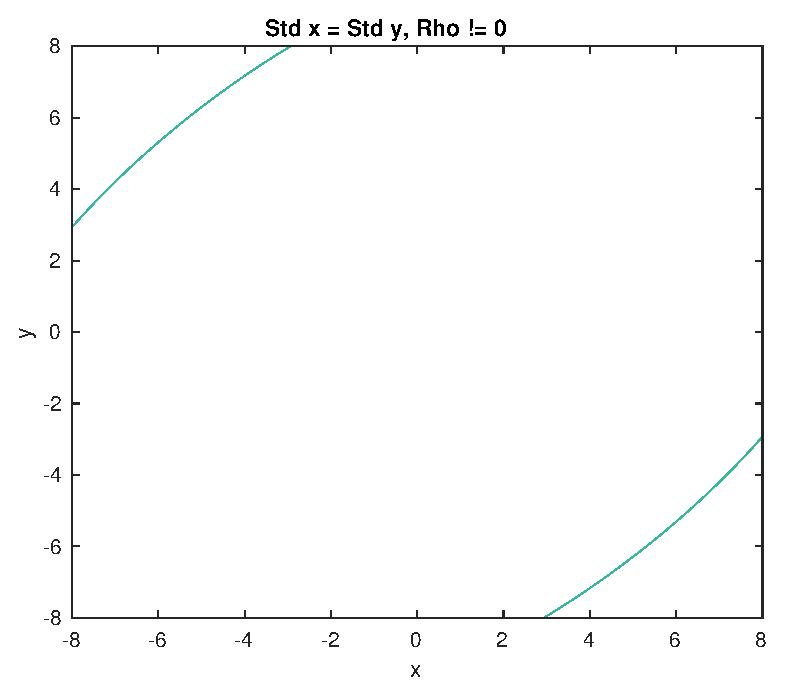
\includegraphics [width=4in]{prob_5_75_04.eps}


\subsection*{E}

\begin{verbatim}
stdx = 3; stdy = 3;
varx = stdx^2; vary=stdy^2;
rho = 0;

X1 = (X-mux)/stdx;
Y1 = (Y-muy)/stdy;

Z = X1.^2-2*rho*X1.*Y1+Y1.^2;
c = [.1 .5 1 2 4 8];

figure(5);
contour(X,Y,Z,c)

title('Std x = Std y, Various C');
xlabel('x'); ylabel('y');
\end{verbatim}

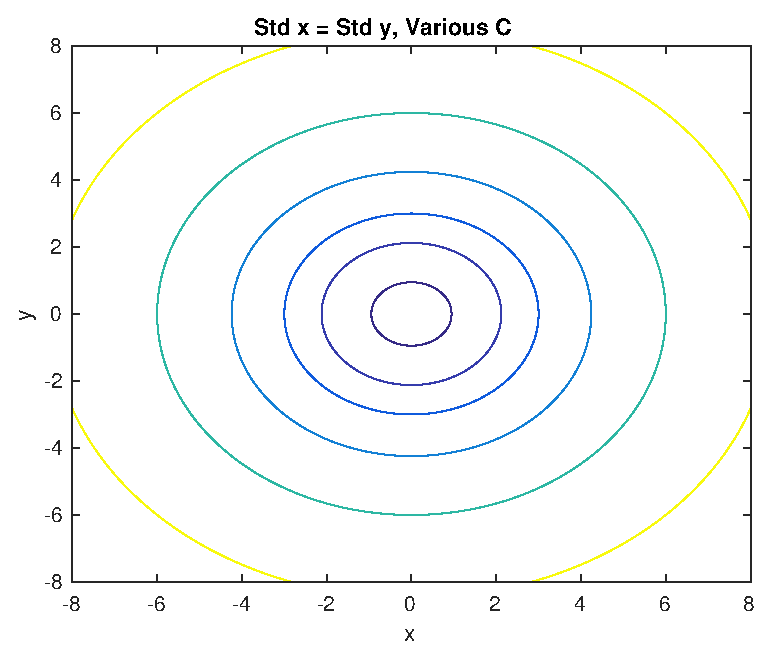
\includegraphics [width=4in]{prob_5_75_05.eps}

\section*{Problem 5.77}


\subsection*{Contents}

\begin{itemize}
\setlength{\itemsep}{-1ex}
   \item Setup
   \item Experiment
   \item Theory
\end{itemize}


\subsection*{Setup}

\begin{verbatim}
clear; close all; clc

trials = 1000000;

X = randn(trials,1) + 1; % Mean 1 - Variance = 1
Y = randn(trials,1); % Mean = 0 - Variance = 1
\end{verbatim}


\subsection*{Experiment}

\begin{verbatim}
hits = sum((X.^2 + Y.^2) <= 1,1);
p_exp = hits/trials;
\end{verbatim}


\subsection*{Theory}

\begin{verbatim}
fxy = @(x,y) (1/(2*pi)).*exp(-((x.*cos(y)-1).^2+(x.*sin(y)).^2)./2).*x;

p_theory = integral2(fxy,0,1,0,2.*pi);


disp(p_exp);
disp(p_theory);
\end{verbatim}

        \color{lightgray} \begin{verbatim}    0.2671

    0.2671

\end{verbatim} \color{black}

\end{document}
